\section{Generalized VPN problem}
To describe the generalized VPN problem, we first describe the class of tree demands.
Let $G = (V_G, E_G)$ be the underlying network graph with terminal set $W \subseteq V_G$.
Let an edge-capacitated tree $T = (V_T, E_T)$ be given with leaf set exactly the terminals $W$, and edge capacities $b_e$ for $e \in E_T$.
Then $T$ describes the tree demand universe $\mathcal U_T$ where a symmetric demand matrix $(D_{ij})$ belongs to $\mathcal U_T$ when it can be routed on $T$.
That is, for all edges $e$ on the (unique) path $\pi_T(i,j)$ between $i$ and $j$ in $T$ it must hold that $D_{ij} \le b_e$.
Note that if we take $T$ to be a star with center $r$ and edge capacities $b_{ir} = b_i$, then $\mathcal U_T$ describes the same universe as the hose model $\mathcal H$ with marginal demands $b_i$.
Hence, tree demands indeed generalize the hose model.

The generalized VPN is now fully characterized by the underlying network graph $G$, a terminal set $W$, edge per-unit-capacity costs $c_e$ ($e \in E_G$), and the \emph{demand tree} $T$ with edge capacities $b_f$ ($f \in E_T$).
A solution to the problem consists of a routing template $\mathcal P = \set{P_{ij} : i,j \in \binom W 2}$ and bought edge capacities $x_e$ for all $e \in E_G$.
We call a solution \emph{feasible} when all demand matrices in $\mathcal U_T$ can be routed on $G$ according to the routing template and without exceeding the installed edge capacities $x$.
We furthermore call a solution optimal if it is feasible and minimizes $\sum_{e \in E_G} c_e x_e$.

\subsection{Integer programming formulation}
The generalized VPN problem can be formulated as the integer program~\eqref{eq:gvpn:mip:semiinf:obj}--\eqref{eq:gvpn:mip:semiinf:f}.
\begin{alignat}{5}
    \text{minimize}\ && \sum_{uv \in E_G} c_{uv} \cdot x_{uv} &&& \label{eq:gvpn:mip:semiinf:obj}\\
    \text{subject to}\ && x_{uv} &\ge \sum_{ij \in \binom{W}{2}} D_{ij} \cdot (f_{uv}^{ij} + f_{vu}^{ij}) &&\qquad \forall_{uv \in E_G,\ D \in \mathcal U_T} \label{eq:gvpn:mip:semiinf:demand}\\
    && \sum_{uv \in \delta(u)} (f_{uv}^{ij} - f_{vu}^{ij}) &= \begin{cases}
                                                                  1 & \text{if $u = i$} \\
                                                                  -1 & \text{if $u = j$} \\
                                                                  0 & \text{otherwise}
    \end{cases} &&\qquad \forall_{u \in V_G,\ ij \in \binom{W}{2}} \label{eq:gvpn:mip:semiinf:flow}\\
    && x_{uv} &\in \mathbb{R}_+ &&\qquad \forall_{uv \in E_G} \label{eq:gvpn:mip:semiinf:x}\\
    && f_{uv}^{ij},\ f_{vu}^{ij} &\in \{ 0, 1 \} &&\qquad \forall_{uv \in E_G,\ ij \in \binom{W}{2}} \label{eq:gvpn:mip:semiinf:f}
\end{alignat}
Each edge $uv$ has constant cost $c_{uv}$ and has a non-negative variable $x_{uv}$ indicating the bought capacity for this edge.
The objective is then to minimize the total cost, i.e.\ the sum of $c_{uv} x_{uv}$ over all edges $uv$.

For each unordered pair of terminals $\set{i, j} \in \binom W 2$, a routing path between these terminals is constructed using binary flow variables.
The flow variable $f_{uv}^{ij}$ indicates whether the directed edge $(u, v)$ is used on the path from terminal $i$ to $j$.
This can be modeled with traditional flow constraints in constraint~\eqref{eq:gvpn:mip:semiinf:flow}.
The routing path from $i$ to $j$ is then given by the set of directed edges $\set{(u, v) \in E_G | f_{uv}^{ij} = 1}$.
By symmetry, we only need to consider one ordering of all unordered pairs.
For ease of notation, we will still describe flow variables with $f_{uv}^{ij}$.

Constraint~\eqref{eq:gvpn:mip:semiinf:demand} ensures that we buy enough capacity on each edge.
For a demand matrix $D \in \mathcal U_T$, we can derive the required capacity on an edge $uv$ using the flow variables.
If $f^{ij}_{uv}$ or $f^{ij}_{vu}$ is 1, then we must buy $D_{ij}$ capacity on edge $uv$ to facilitate the flow between terminals $i$ and $j$.
Thus, we obtain the constraint
\[
    x_{uv} \ge \sum_{ij \in \binom W 2} D_{ij} ( f^{ij}_{uv} + f^{ij}_{vu}),
\]
which must hold for any edge $uv$ and for any demand matrix $D_{ij} \in \mathcal U_T$.

This definition leads to an infinite number of constraints as $\mathcal U_T$ is in general not a finite set of matrices.
This issue can be resolved with row generation, where we solve the program by only considering a subset $\mathcal U_T^* \subset \mathcal U_T$ in constraint~\eqref{eq:gvpn:mip:semiinf:demand}.
Then we obtain a solution $(\tilde x, \tilde f)$ that is only valid for all $D \in \mathcal U_T^*$.
We then assess whether there exists a matrix $D \in \mathcal U_T \setminus \mathcal U_T^*$ that violates the constraint.
If such a matrix exists, we add it to $\mathcal U_T^*$ and solve the program again until we cannot find any violating matrix.
Note that a violating matrix $D$ satisfies
\[
    \tilde x_{uv} < \sum_{ij \in \binom W 2} D_{ij} \cdot (\tilde f^{ij}_{uv} + \tilde f^{ij}_{vu})
\]
for some edge $uv \in E_G$.
We can thus find such a violating matrix by solving the following linear subproblems, one for each $uv \in E_G$:
\begin{alignat*}{5}
    p_{uv} = \text{maximize}\quad && \sum_{ij \in \binom{W}{2}} (\tilde f_{uv}^{ij} + \tilde f_{vu}^{ij}) \cdot D_{ij} &&& \\
    \text{subject to}\quad && \sum_{\substack{ij \in \binom{W}{2}\\e \in \pi_T(i,j)}} D_{ij} &\le b_e &&\qquad \forall_{e \in E_T} \\
    && D_{ij} &\in \mathbb{R}_+ &&\qquad \forall_{ij \in \binom{W}{2}}
\end{alignat*}
If for any of these subproblems the optimal solution $D^*$ has objective $p_{uv} > \tilde x_{uv}$, we add $D^*$ to $\mathcal U_T^*$.
Otherwise, $\mathcal U_T^*$ was representative for $\mathcal U_T$ and we can conclude that the integer program~\eqref{eq:gvpn:mip:semiinf:obj}--\eqref{eq:gvpn:mip:semiinf:f} is optimal.

Although the row generation subproblems do not contain integer variables, the overall procedure to find an optimal solution for \eqref{eq:gvpn:mip:semiinf:obj}--\eqref{eq:gvpn:mip:semiinf:f} may use a large number of iterations.
Using a clever dualization trick (also performed in~\cite{altin2007provisioning}) we can obtain a compact MIP formulation that does not require row generation.

For this trick, consider a single edge $uv \in E_G$ and consider $f$ as parameters.
Note that we can write constraint~\eqref{eq:gvpn:mip:semiinf:demand} as
\[
    x_{uv} \ge \max_{D \in \mathcal U_T} \sum_{ij \in \binom W 2} D_{ij} \cdot (f^{ij}_{uv} + f^{ij}_{vu}),
\]
or, when writing out the polyhedral constraints describing $\mathcal U_T$, as the optimization problem
\begin{alignat}{5}
    x_{uv} \ge \text{maximize}\ && \sum_{ij \in \binom{W}{2}} (f_{uv}^{ij} + f_{vu}^{ij}) \cdot D_{ij} &&& \\
    \text{subject to}\ && \sum_{\substack{ij \in \binom{W}{2}\\e \in \pi_T(i,j)}} D_{ij} &\le b_e &&\qquad \forall_{e \in E_T} \label{eq:gvpn:dualtrick} \\
    && D_{ij} &\in \mathbb{R}_+ &&\qquad \forall_{ij \in \binom{W}{2}}
\end{alignat}
Since this linear program is feasible and bounded, we might just as well write the dual
\begin{alignat}{5}
    x_{uv} \ge \text{minimize}\ && \sum_{e \in E_T} b_e \cdot \omega_e^{uv} &&& \label{eq:gvpn:dualtrick:min} \\
    \text{subject to}\ && \sum_{e \in \pi_T(i,j)} \omega_e^{uv} &\ge f_{uv}^{ij} + f_{vu}^{ij} &&\qquad \forall_{ij \in \binom{W}{2}} \\
    && \omega_e^{uv} &\in \mathbb{R}_+ &&\qquad \forall_{e \in E_T}
\end{alignat}
where $\omega_e^{uv}$ are the  dual variables for constraint~\eqref{eq:gvpn:dualtrick}.
Now, note that we can drop the minimize in \eqref{eq:gvpn:dualtrick:min} as the objective function of the original MIP is a non-negatively weighted sum of the variables $x_{uv}$.
We now have thus obtained a compact MIP formulation for the generalized VPN problem:
\begin{alignat*}{5}
    \text{minimize}\ && \sum_{uv \in E_G} c_{uv} \cdot x_{uv} &&& \\
    \text{subject to}\ && x_{uv} &\ge \sum_{e \in E_T} b_e \cdot \omega_e^{uv} &&\qquad \forall_{uv \in E_G} \\
    && \sum_{e \in \pi_T(i,j)} \omega_e^{uv} &\ge f_{uv}^{ij} + f_{vu}^{ij} &&\qquad \forall_{uv \in E_G,\ ij \in \binom{W}{2}} \\
    && \sum_{uv \in \delta(u)} (f_{uv}^{ij} - f_{vu}^{ij}) &= \begin{cases}
                                                                1 & \text{if $u = i$} \\
                                                                -1 & \text{if $u = j$} \\
                                                                0 & \text{otherwise}
    \end{cases} &&\qquad \forall_{u \in V_G,\ ij \in \binom{W}{2}} \\
    && x_{uv} &\in \mathbb{R}_+ &&\qquad \forall_{uv \in E_G} \\
    && \omega_e^{uv} &\in \mathbb{R}_+ &&\qquad \forall_{uv \in E_G,\ e \in E_T} \\
    && f_{uv}^{ij},\ f_{vu}^{ij} &\in \{ 0, 1 \} &&\qquad \forall_{uv \in E_G,\ ij \in \binom{W}{2}}
\end{alignat*}

\subsection{Hierarchical hubbing algorithm}
\begin{algorithm}[t]
    \caption{RecursiveHubbing}
    \label{alg:bruteForceHubbing}
    \begin{algorithmic}[1]
        \Statex Recursive enumeration algorithm to find all optimal mappings. Initially, verticesToAssign equals $V_T - W$ and $h$ is an empty mapping from $V_T$ to $V_G$. In the actual implementation, we also maintain a set of all best mappings that attain the minimum cost.

        \Procedure{Assign}{verticesToAssign, $h$}
            \If {verticesToAssign is empty}
                \State \Return $\sum_{uv \in E_T} d(h(u), h(v))$ \Comment{The cost of mapping $h$}
            \EndIf

            \State $u \gets$ verticesToAssign.first()
            \State bestCost $\gets \infty$

            \ForAll {vertices $v$ in graph}
                \State $h(u) \gets v$
                \State currentCost $\gets$ \textsc{Assign}(verticesToAssign $-$ $u$, $h$)

                \If {currentCost $<$ bestCost}
                    \State bestCost $\gets$ currentCost
                \EndIf
            \EndFor

            \State \Return bestCost
        \EndProcedure
    \end{algorithmic}
\end{algorithm}

Olver and Shepherd suggested an 8-approximation algorithm for this problem~\cite{olver2010approxrnd}.
They considered the optimal solution over all \emph{hubbing solutions}.
A hubbing solution maps each internal node in the demand tree to a vertex in $V_G$.
Each terminal must be mapped to its corresponding vertex in $G$.
This mapping function is denoted with $h$
For each edge $uv$ in the demand tree, we then buy $b_{uv}$ capacity along the shortest path between $h(u)$ and $h(v)$ in the original graph $G$, where each edge $e$ has its cost $c_e$ as weight.
The total cost then becomes
\[
    \sum_{uv \in E_T} b_{uv} d_c(h(u), h(v)),
\]
where $d_c(h(u), h(v))$ gives the distance between $h(u)$ and $h(v)$ in $G$ where $c$ defines the edge weights.
It was conjectured that this algorithm is optimal, i.e.\ that an optimal hubbing solution is an optimal solution for the generalized VPN problem.

Algorithm~\ref{alg:bruteForceHubbing} describes a recursive algorithm to find the optimal hubbing solution.
With a standard recursive approach, the total cost is calculated for each mapping $h$ from $V_T \setminus W$ to $V_G$.
The optimal cost is then returned; notice that the actual mapping can easily be returned as well.
From this mapping, the routing templates can be derived.

However, it is possible to determine the optimal hubbing solution more efficiently using dynamic programming~\cite{olver2010approxrnd}.
We first pick an arbitrary internal node of the demand tree as root.
Then we root the demand tree here.
A subtree of this tree is a tree that is rooted at a vertex in this tree, i.e.\ a vertex and all nodes below it.
This tree has a parent (unless it is the entire tree) and children (unless the root is a terminal).
Algorithm~\ref{alg:subtrees} derives the set of subtrees, denoted by $\mathcal L$, in a BFS manner.

For any subtree $S \in \mathcal L$ and vertex $v \in V_G$, we consider the subproblem $C[S, v]$.
It stores the cost of an optimal hubbing solution of the problem restricted to subtree $S$, where the root of $S$ is mapped to $v$.
The final solution is then $\min_{v \in V_G} C[T, v]$.

Let $S_w$ denote the subtree rooted at a vertex $w \in T$.
Now suppose that we want to obtain the value for $C[S_r, v]$ for some vertex $r \in V_T$ and $v \in V_G$, while $C[S_{r_i}, w]$ is known for all children $r_i$ of $r$ and all vertices $w \in V_G$.
Then the mappings of the subtrees are independent of each other.
The contribution of one specific subtree $S_{r_i}$ to the cost of subtree $S_r$ is
\[
    \min_{w \in V_G} \set{C[S_{r_i}, w] + b_{r, r_i} d_c(v, w)}.
\]
Notice that the mapping of $r$ is $v$ and the mapping of $r_i$ is $w$ in this recurrence.
We minimize the cost of this subtree over all possible choices for $w$.
This gives the following recurrence.
\[
    C[S_r, v] = \begin{cases}
                  0 &\text{if $r \in W$ and $r = v$,} \\
                  \infty &\text{if $r \in W$ and $r \neq v$,} \\
                  \displaystyle \sum_{\text{children $r_i$ of $r$}} \min_{w \in V_G} \set{ C[S_{r_i}, w] + b_{r, r_i} d(v, w) } &\text{otherwise.} \\
    \end{cases}
\]

\begin{algorithm}[t]
    \caption{Finding all subtrees for the dynamic programming algorithm}
    \label{alg:subtrees}
    \begin{algorithmic}[1]
        \Statex Obtaining all subtrees that are needed for the dynamic programming algorithm.
        The dynamic program itself only fills in the table based on the recurrence stated below.
        \Procedure{GetSubtrees}{$V_T, E_T, W$}
            \State root = arbitrary node in $V_T - W$

            \State $\mathcal L \gets \emptyset$
            \State $S \gets$ Subtree(root, root.neighbors, null) \Comment{A subtree has a root, children and parent}
            \State $\mathcal L$.add($S$)
            \State $\mathcal Q$.add($S$)

            \While {$\mathcal Q$ is not empty}
                \State tree $\gets \mathcal Q$.removeFirst()
                \State currentRoot $\gets$ tree.root
                \ForAll{vertices $r$ in tree.children}
                    \State $S$ = Subtree($r$, $r$.neighbors $-$ currentRoot, currentRoot)
                    \State $\mathcal L$.add($S$)
                    \State $\mathcal Q$.add($S$)
                \EndFor
            \EndWhile
            \State \Return subtrees.reversed()
        \EndProcedure
    \end{algorithmic}
\end{algorithm}

\subsection{Experiments}
Using the implementation of the exact MIP formulation (using Gurobi) and the dynamic programming solution with hubs, we tried to find instances where the optimal solutions have different objective values.
That would be a counterexample for the conjecture that the dynamic programming algorithm is optimal.
We are also interested in instances where the LP relaxation leads to an integrality gap, because %TODO mag Sten uitleggen. %TODO waarom ookalweer

\subsubsection{The Petersen graph with a 2-union star}
In our first experiments, we considered the Petersen graph with unit edge cost as the network $G$.
We construct an instance as follows.
The demand tree $T$ is a \emph{two-union star}, that is, two star graphs where the centers are connected by an edge.
We considered all possible sets of terminals $W \subseteq V_G$.
For a set of terminals $W$, we considered all partitions of $W$ into $W_1$ and $W_2$.
Then all terminals in $W_1$ are connected to an internal vertex and all terminals in $W_2$ are connected to another internal vertex (creating two stars).
The two internal vertices are connected with an edge, called the \emph{bridge}.

This leads to a total of $68\,185$ instances.
None of these gave a counterexample for the conjecture, nor did any instance yield an integrality gap for the integer program.

\subsubsection{Randomized Petersen experiments}\label{subsubsec:random}
In the following series of experiments, we again considered the Petersen graph as network $G$.
However, we assigned randomized edge costs now, rather than using unit costs.
The edge costs were sampled uniformly from $[1, 10]$.
Each vertex was picked with probability $1/2$ as terminal while ensuring that there are at least four terminals.
Otherwise, the demand tree reduces to a star and the instance is equivalent to a regular VPN problem instance.

Lastly, a demand tree is constructed that has the set terminals as leaves.
The number of internal nodes is sampled uniformly from $[3, |W|]$, where $W$ is the set of terminals.
Then a spanning tree is randomly constructed on the internal nodes.
The demand tree is then created by connecting each terminal to an arbitrary internal node and removing internal nodes that are leaves.
The capacities of the edges in the demand tree are sampled from a geometric distribution with success probability $0.4$.

Over $100\,000$ instances were generated, but none of these resulted in a counterexample nor an integrality gap.

\subsubsection{The augmented Petersen graph}
For these experiments, the network $G$ is the \emph{augmented Petersen graph}.
This graph is defined as the Petersen graph with unit edge costs and an additional vertex.
This additional vertex is connected to all vertices with an edge of cost 2.
The terminals are the ten original vertices of the Petersen graph.

The structure of the demand tree is shown in Figure~\ref{fig:augpetersen}.
The tree has a (terminal) root node and a center node.
These two vertices are connected with an edge of capacity either $3$, $5$ or $\infty$.
Then we are going to pick groups of terminals.
For each edge $uv$ of the original Petersen graph, we create a group of three vertices.
First, one endpoint is picked, say $u$, and then its two neighbors other than $v$ are added.
This gives a group of three vertices and we create such a group for each of the fifteen edges of the Petersen graph.
For each group, we add three new leaves to the demand tree, connect them with weight 1 to a new interior node, and connect the interior node to the center with capacity $1$, $2$ or $3$.

\begin{figure}
    \centering
    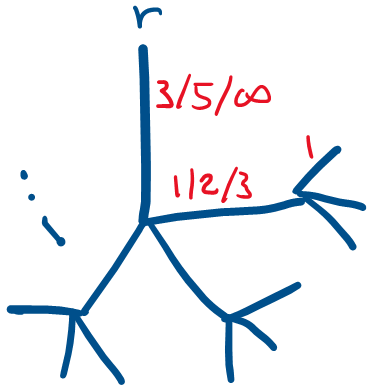
\includegraphics[width=0.2\textwidth]{augpetersen}
    \caption{Structure of the demand tree for the augmented Petersen graph instances.}
    \label{fig:augpetersen}
\end{figure}

For each of the nine suggested combinations of capacities in the demand tree, we considered 200 sets of fifteen groups.
None yielded a counterexample nor an integrality gap.
Similarly, we also tried adding two groups for each edge (one for each endpoint), but this did not yield any results either.

\subsubsection{Realistic VPN instances}
We also considered realistic VPN instances, as provided by Laura, as network $G$.
The construction of the demand tree was randomized, similarly to the experiments in Section~\ref{subsubsec:random}.
The edge weight of an edge that connects to a terminal is the provided terminal capacity.
Capacities of edges between internal nodes are sampled from a normal distribution with as parameters the sample mean and sample variance of the terminal capacities.
As these instances have more vertices and many more terminals than the other instances, the solving the integer program requires an considerable amount of time and resources.
We therefore only considered a few instances, but these did not result in counterexamples or integrality gaps.

\subsubsection{Integrality gap instances}
Together with their proof of the VPN conjecture, Goyal, Olver and Shepherd provided instances that gave an integrality gap for the VPN problem~\cite{goyal2013vpn}.
We used a 2-union star as demand tree, where we tried all partitions of the terminals into these two halves and all relevant integer capacities of the bridge (i.e., not reducing to the original VPN problem).
Notice that the original VPN instances did have an integrality gap.
The result were interesting.
We considered the graph with six terminals.
For a partition with two terminals on one side and four on the other, and a bridge capacity of $1$, there was no integrality gap.
However, for three terminals on both sides, we do see an integrality gap for a bridge capacity of 1 or 2.
We observed the same behavior for larger instances: if one half has only two terminals, there is no integrality gap for a bridge capacity of $1$.
However, when both sides have at least three terminals, there is an integrality gap.
This lead to the idea that the generalized VPN problem might be easier on 2-union stars where one half only has two terminals.
An attempt to prove that the conjecture holds in this situation will follow in the next paragraph.

\subsection{The generalized VPN conjecture on ring networks} \label{subsec:genvpn:rings}
The paper by Grandoni et al.~\cite{grandoni2008short} gives a short proof that the VPN conjecture is true for the cases where $G$ is a ring.
In this section, we will discuss an attempt to extend the proof to the generalized VPN conjecture, for the cases where the network is a ring and the demand tree is a \emph{two-union star}: the tree formed by connecting the centers of two star graphs.
We refer to this edge between the centers as the bridge.

As mentioned in \cite{grandoni2008short}, the hubbing solution that is computed by the polynomial-time algorithm is also a \emph{tree solution}, that is, the support of the routing template forms a tree.
Exploiting this structure is key for the argument to work.
In the generalized setting however, the hierarchical hubbing solution may not be a tree solution, even in the restricted case of the ring network with a two-union star demand tree.
A small counterexample is given in Figure~\ref{fig:counterex-tree-solution}.
In any optimal hubbing solution, the internal node $R^+$ needs to be mapped to either to the site of $B^+$ or $C^+$ in $G$.
Symmetrically, $R^-$ needs to be mapped to either $B^-$ or $C^-$.
The optimal hubbing solution is then no tree solution, as the shortest path between the mapped $R^+$ and $R^-$ uses the bottom edge between $C^+$ and $C^-$, while the shortest path between the mapped $R^+$ and $A^+$ goes via $A^-$, and likewise the shortest path between the mapped $R^-$ to $A^-$ goes via $A^+$.
Indeed, the support of the routing template is the whole cycle $G$.

\begin{figure}
    \centering
    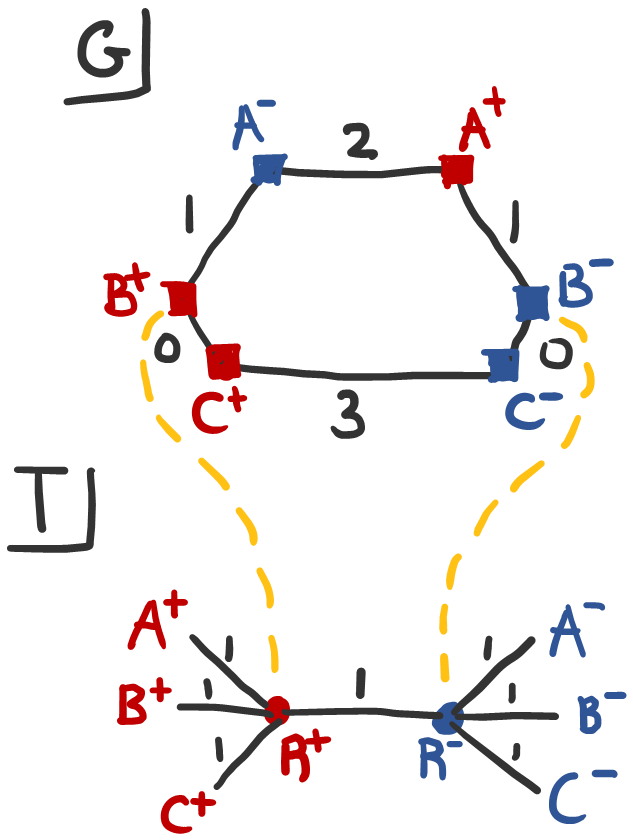
\includegraphics[width=.3\textwidth]{counterexample-tree-solution}
    \caption{Counterexample that the optimal hubbing solution is a tree solution.} \label{fig:counterex-tree-solution}
\end{figure}

The above counterexample uses a demand tree with (at least) three terminals at either side of the two-union star, and one might wonder what happens for the case where there are only two terminals on one side (notice that the case is solved when having only one terminal, as then the demand tree reduces to a star).
With a slightly different construction as in Figure~\ref{fig:counterex2}, we see that no tree solution is guaranteed here either. % TODO: explanation

\begin{figure}
    \centering
    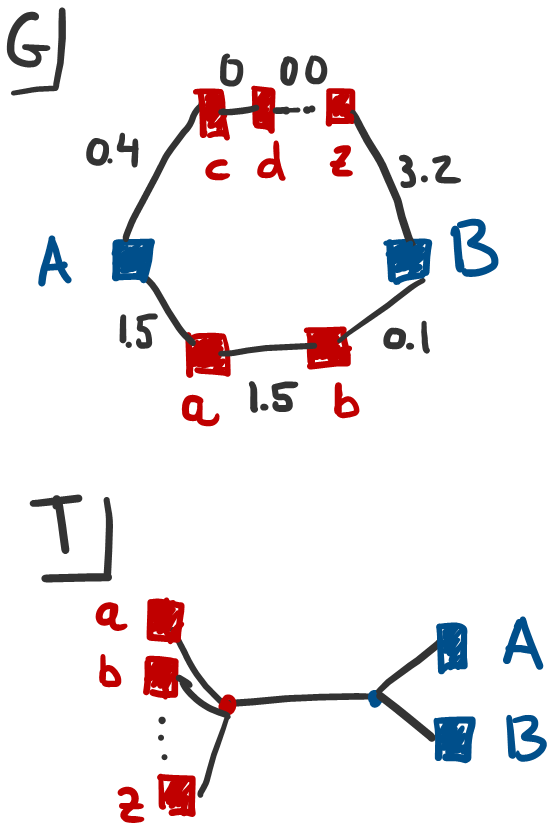
\includegraphics[width=.3\textwidth]{counterexample2}
    \caption{Counterexample that the optimal hubbing solution is a tree solution, when one side of the demand tree has only two terminals.}
    \label{fig:counterex2}
\end{figure}

These counterexamples make our initial efforts of constructing a `generalized' pyramidal routing problem (the equivalent of the pyramidal routing problem in \cite{grandoni2008short}) not generally applicable, as the construction relies on the existence of a tree solution.
Some insights we gained might be useful for more compelling attempts of proving the generalized conjecture;
they can be found in Appendix~\ref{app:proof}.
